% !TEX root = ../Dissertation.tex
%===================================================================================================

\chapter{Chapter 3 Title}

\Cref{fig:ODonnellE1986-f42-1} is drawn entirely in tikz.

\begin{figure}[h!]
	\centering
	%\includegraphics[width=0.7\textwidth]{Figures/ODonnellE1986-f42-1.pdf}
	%\tikzset{external/remake next}
	\tikzsetnextfilename{ODonnelE1986}
	\begin{tikzpicture}[trim axis left]	
		\begin{axis}[
			box plot axis,
			width=0.6\textwidth,
			height=0.6\textwidth,
			xmin=0,
			xmax=1,
			ymin=0,
			ymax=1.1,
			xtick={0.1,0.9},
			ytick={0.1,0.9},
			xticklabels={Low,High},
			yticklabels={Low,High},
			enlargelimits=false,
			ytick style={/pgfplots/major tick length=0pt,},
			xtick style={/pgfplots/major tick length=0pt,},
			ylabel=Level of operator performance,
			xlabel=Level of operator workload,
			];
			
			\draw (axis cs: 0.3,1.1) -- (axis cs: 0.3,1);
			\draw (axis cs: 0.7,1.1) -- (axis cs: 0.7,1);
			
			\draw[blue,line width=1pt] (axis cs: 0,0.9) -- (axis cs: 0.3, 0.9) .. controls (axis cs: 0.6,0.9) and (axis cs: 0.7,0.6)  .. (axis cs: 0.7,0.2) -- (axis cs: 1,0.2);
			\draw (axis cs: 0.15,1) node[anchor=south] {\large A};
			\draw (axis cs: 0.5,1) node[anchor=south] {\large B};
			\draw (axis cs: 0.85,1) node[anchor=south] {\large C};

		\end{axis}
	\end{tikzpicture}

	\caption[Hypothetical relationship between workload and operator performance]{Hypothetical relationship between workload and operator performance
	proposed to depend upon the relative level of operator workload. Reproduced
	from \citet[][Fig 42.1]{ODonnellE1986}.}
	\label{fig:ODonnellE1986-f42-1}
\end{figure}

\Cref{fig:nexus} has lots of subfigures.

\begin{figure}
	\centering
	\begin{subfigure}{\textwidth}
		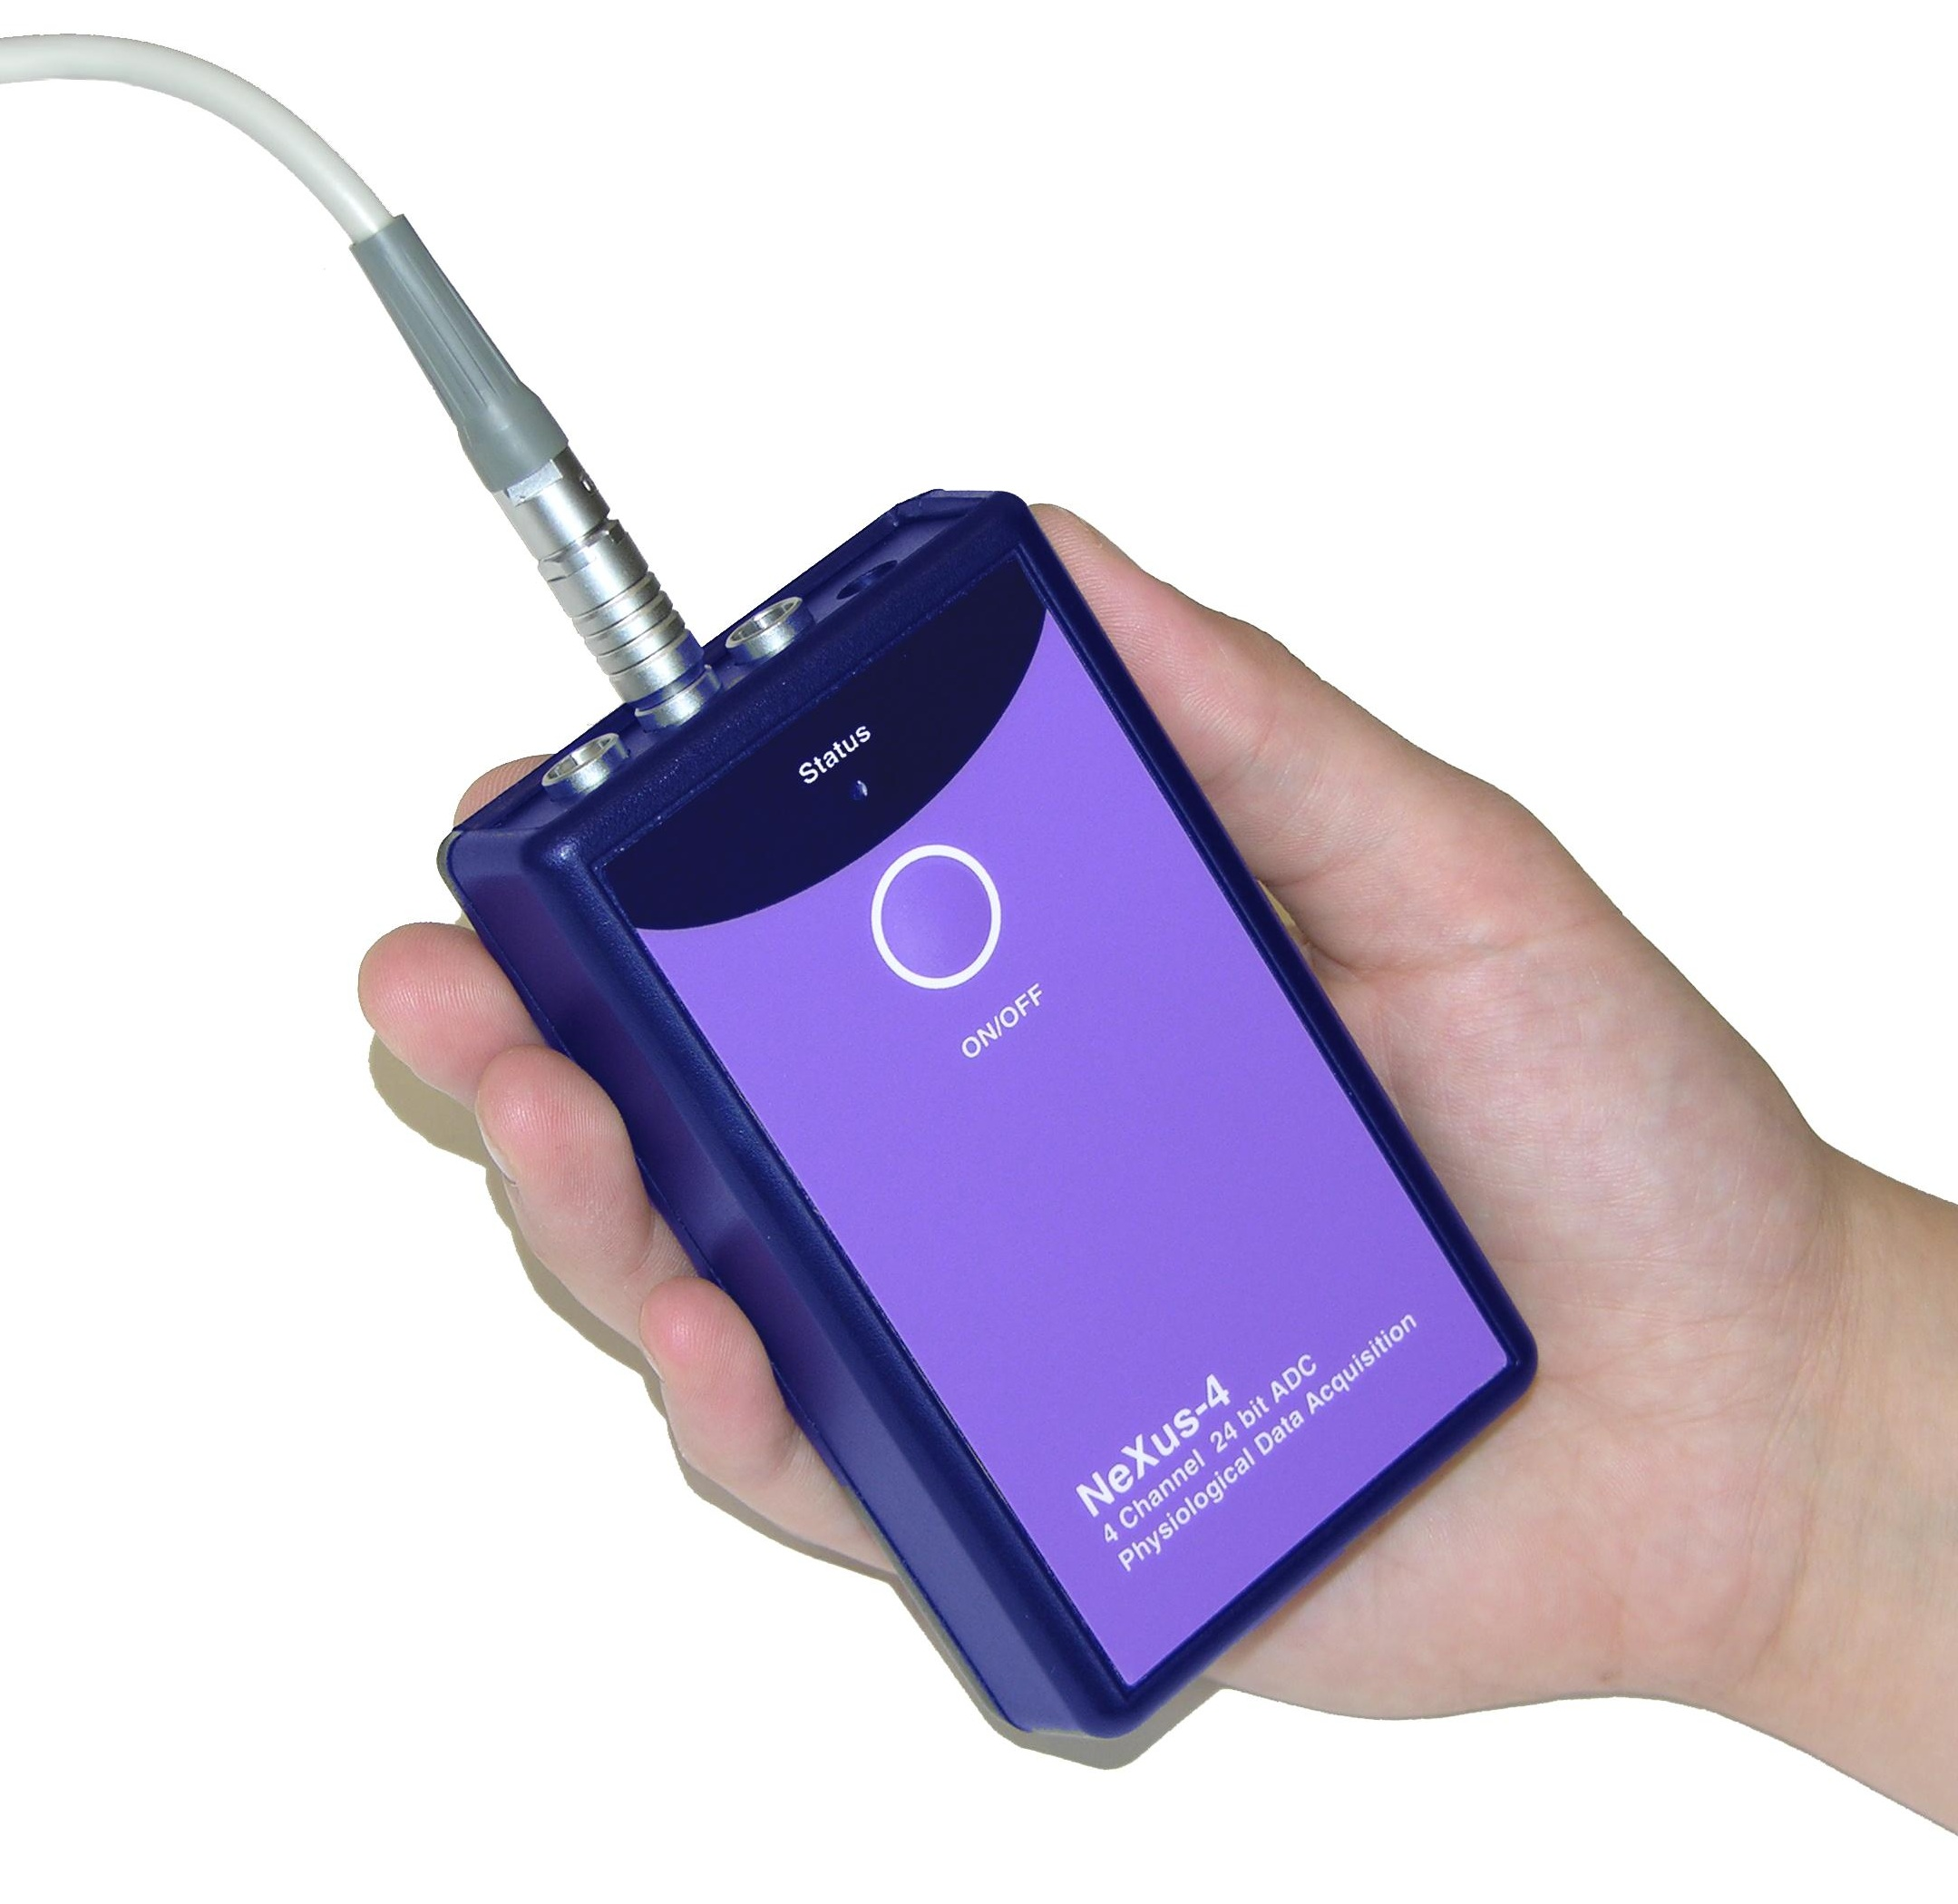
\includegraphics[width=\textwidth] {Figures/nexus.jpg}
		\caption{The Nexus-4 device}
	\end{subfigure}
	
	\vspace{10mm}
	\begin{subfigure}{0.41\textwidth}
		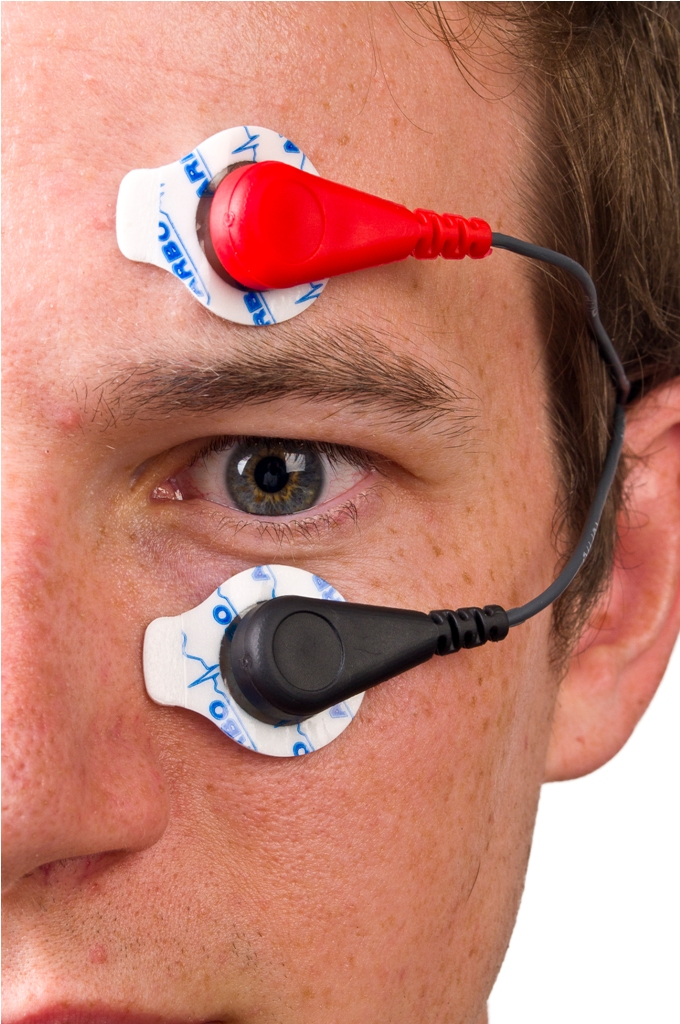
\includegraphics[width=\textwidth] {Figures/nexusEOG.jpg}
		\caption{EOG Sensor}
	\end{subfigure}
	\hfill
	\begin{tabular}{c}
		\begin{subfigure}{0.45\textwidth}
			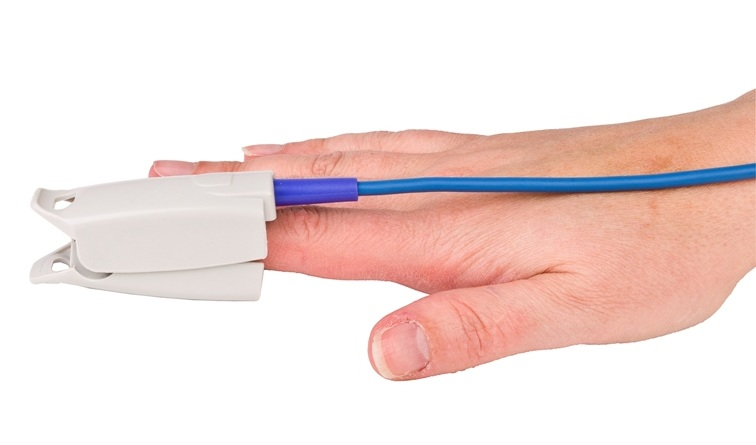
\includegraphics[width=\textwidth] {Figures/nexusBVP.jpg}
			\caption{BVP Sensor}
		\end{subfigure}
		\\
		\begin{subfigure}{0.45\textwidth}
			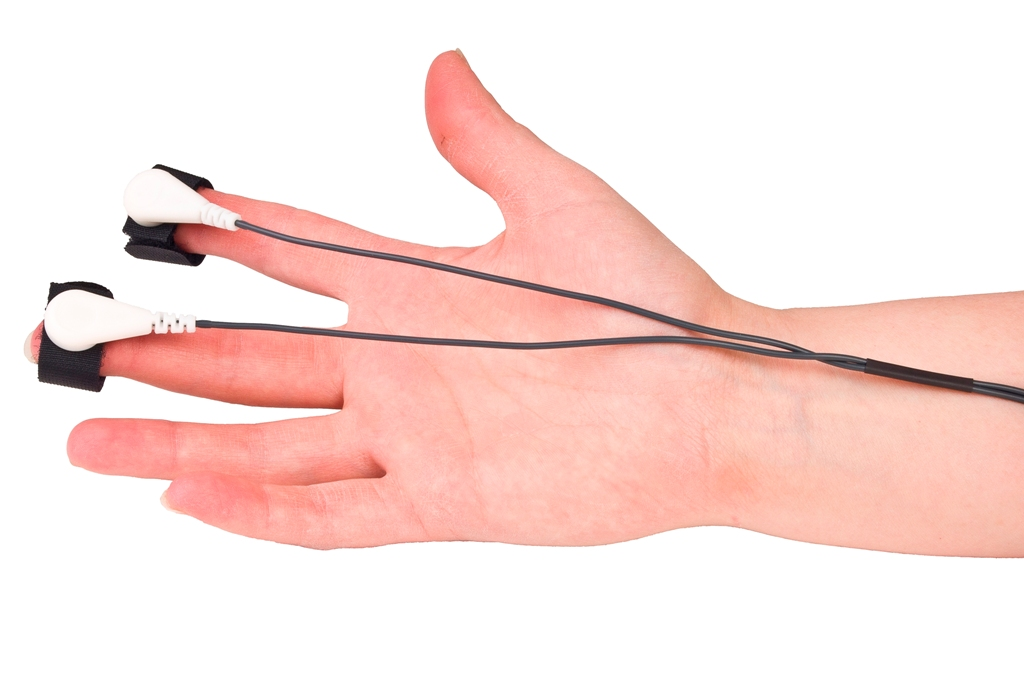
\includegraphics[width=\textwidth] {Figures/nexusSC.jpg}
			\caption{SC Sensor}
		\end{subfigure}
	\end{tabular}
	\caption{The Nexus-4 Wireless Physiological Monitoring System}
	\label{fig:nexus}
\end{figure}

\Cref{fig:laterResponse} is another nice tikz diagram

\begin{figure}[h]
	\centering
	%\tikzset{external/remake next}
	\tikzsetnextfilename{laterResponse}
	\begin{tikzpicture}
		\draw[dashed,black!50!white, name path=thold] (-0.1,0) node[black, anchor=east] {$S_T$}  -- (10,0);
		\draw[blue, name path=rise] (-0.1,-2) node[black,anchor=east] {$S_0$} -- (3,-2) -- (7,1);
		
		\draw[->] (0,-2.2) -- (0,1);
		
		\node[rotate=90, anchor=south] at (-0.8,-1) {\begin{minipage}{4cm}\centering\smaller Posterior probability that \\ stimulus has appeared \end{minipage}};
		
		\draw[->] (3,-3) node[anchor=east] {\smaller Time} -- (4.5,-3);
		
		\path[fill=red, opacity=0.5, name intersections={of=rise and thold}]
			(intersection-1) circle (5pt);
		\draw[<-] (intersection-1) ++(6pt,-6pt) -- ++(0.8,-0.5) node[black, opacity=1,anchor=west] {\smaller Response};
		
		\draw[<-] (3,-2) ++(-0.1,0.1) -- ++(-0.9,0.8) node[anchor=south] {\smaller Stimulus appears};
	\end{tikzpicture}
	\caption{Example LATER response to a stimulus}
	\label{fig:laterResponse}
\end{figure}


